\documentclass[10pt]{beamer}

\usetheme[progressbar=frametitle]{metropolis}
\usepackage{appendixnumberbeamer}
\usepackage{booktabs}
\usepackage[scale=2]{ccicons}
\usepackage{pgfplots}
\usepgfplotslibrary{dateplot}
\usepackage{xspace}
\newcommand{\themename}{\textbf{\textsc{metropolis}}\xspace}

\title{Propuesta de Tesis}
\subtitle{Análisis multi-criterio de estructuras del Citoesqueleto mediante grafos}
\date{\today}
%\date{}
\author{Leonardo Pizarro}
\institute{Trabajo de Tesis I - Primavera 2018}
% \titlegraphic{\hfill\includegraphics[height=1.5cm]{logo.pdf}}

\begin{document}

\maketitle

%\begin{frame}{Table of contents}
%  \setbeamertemplate{section in toc}[sections numbered]
%  \tableofcontents[hideallsubsections]
%\end{frame}

\section{Contexto}

\begin{frame}[fragile]{Contexto}
\begin{itemize}
    \item Las estucturas alargadas aparecen continuamente en distintas escalas
    \item En distintas formas: Con y Sin Ciclo
    \begin{itemize}
        \item Con Ciclo: Reticulo
        \item Sin Ciclo: Neurona
    \end{itemize}
\end{itemize}
\begin{center}
    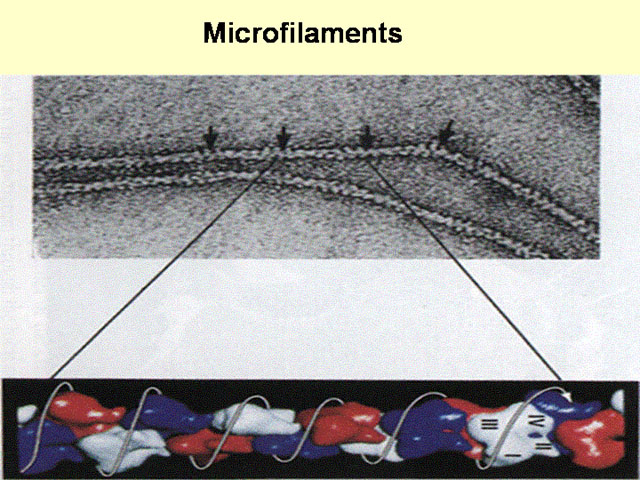
\includegraphics[width=\textwidth,height=0.5\textheight]{nr120.jpg}
        \end{center}
\end{frame}

\begin{frame}[fragile]{Contexto}

\begin{center}
    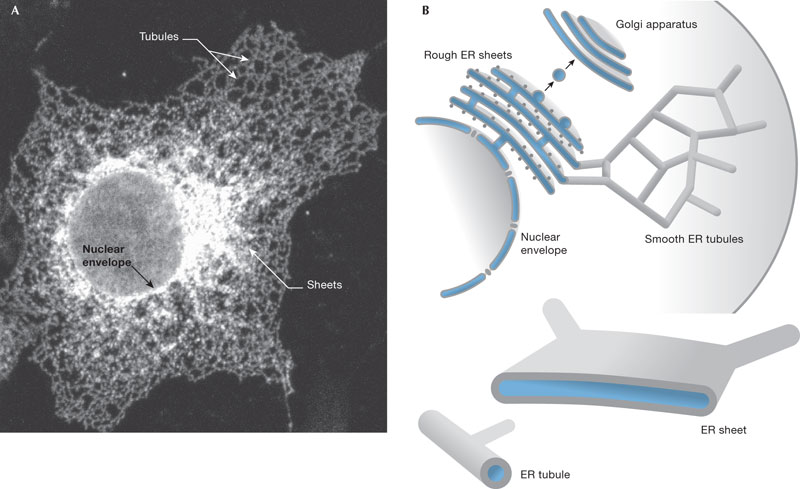
\includegraphics[width=\textwidth]{F1-large.jpg}
        \end{center}
\end{frame}


\begin{frame}[fragile]{Contexto}
\begin{itemize}
    \item Se busca caracterizar mediante la medici\'on de par\'ametros como el largo, ancho, \'angulo predominante, la polaridad.
    \item Existen diversos enfoques:
    \begin{itemize}
        \item An\'alisis de imagen para determinar una red
        \item An\'alisis de imagen para determinar direccionalidad predominante
        \item An\'alisis de imagen para extraer cada uno de los filamentos que componen lo observado
    \end{itemize}
    \item Restricciones del instrumento de observaci\'on
\end{itemize}
\end{frame}

\begin{frame}[fragile]{Microt\'ubulos}
\begin{itemize}
    \item Investigaciones del estado del arte involucran demasiados par\'ametros
\end{itemize}

\begin{center}
    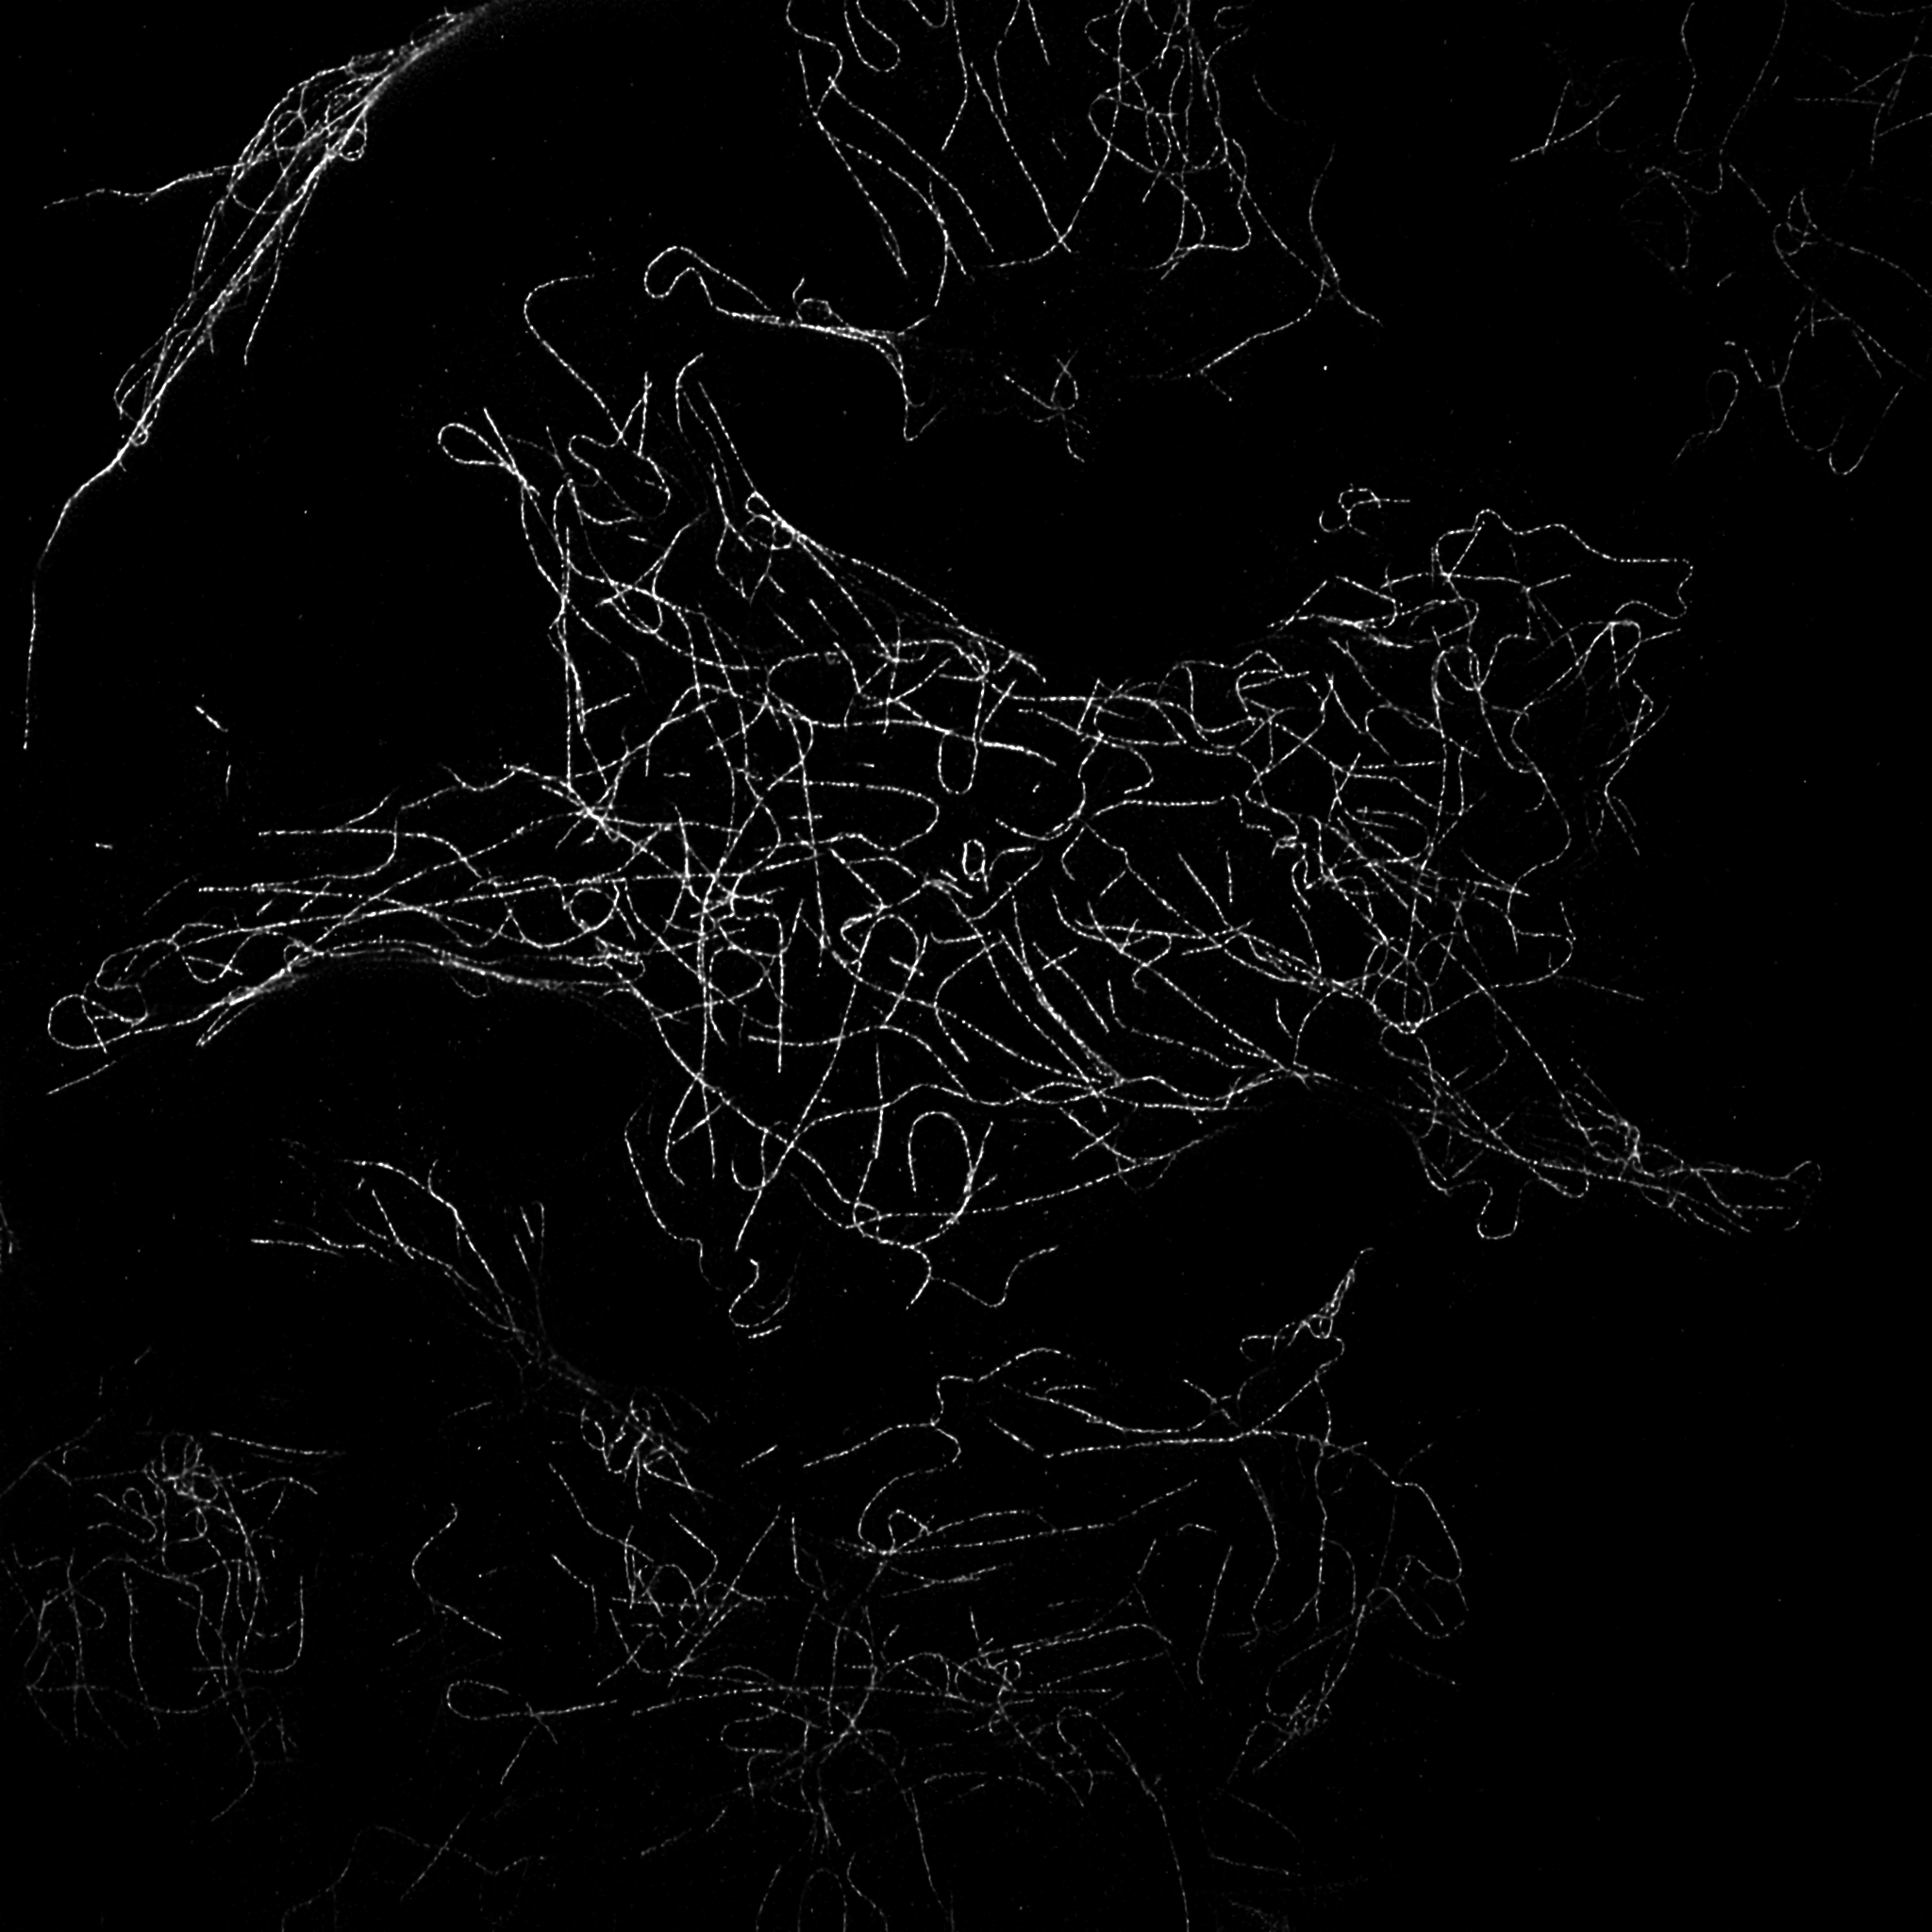
\includegraphics[width=\textwidth]{microtubulos_MAX.png}
        \end{center}
\end{frame}

\begin{frame}[fragile]{Ejemplo base}
\begin{center}
    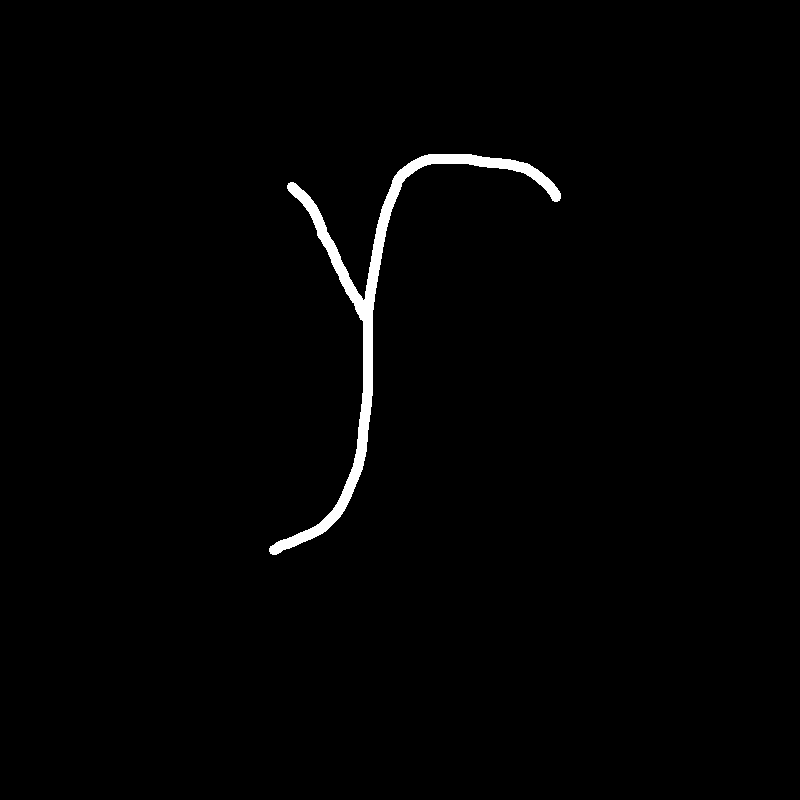
\includegraphics[width=\textwidth,height=0.5\textheight]{test.png}
        \end{center}
\end{frame}

\section{Preguntas de Investigaci\'on}

\begin{frame}{Investigaci\'on}
	Existiendo información a Priori, la que identifica ciertos comportamientos de lo observado (ej: actina no se pega) y comenzando el an\'alisis utilizando im\'agenes con fluorescencia de microfilamentos de celulas eucariotas:
	\begin{itemize}
		\item Cuantos objetos se observan, y que caracter\'isticas/propiedades presentan.
		\item Cual de estas caracter\'isticas es m\'as relevante.
		\item Cual es el costo computacional de una soluci\'on de este tipo.
		\item Cuales son los aspectos relevantes para lograr una generalizaci\'on a otras estructuras alargadas.
	\end{itemize}
\end{frame}

\section{Hip\'otesis}

\begin{frame}[fragile]{Hip\'otesis}

Un enfoque basado en grafos  permite construir una representaci\'on con mayor carga de informaci\'on dados los multi-criterios.

\begin{itemize}
    \item Objetivo 1: Desarrollar un algoritmo que permita incorporar los criterios mencionados previamente. 
\end{itemize}

\end{frame}

\section{Metodolog\'ia}

\begin{frame}{Metodolog\'ia}
  \begin{itemize}
    \item Validar resultados contra criterio \textit{Gold Standard} definido por un experto.
    \item Comparar resultados respecto a la construcci\'on de grafos de m\'etodos con un s\'olo criterios encontrados en la literatura. 
    \item Definir una generalizaci\'on para microt\'ubulos y/o otras estructuras alargadas.
  \end{itemize}
\end{frame}

%\begin{frame}{References}
%  Some references to showcase [allowframebreaks] %\cite{knuth92,ConcreteMath,Simpson,Er01,greenwade93}
%\end{frame}


{\setbeamercolor{palette primary}{fg=black, bg=yellow}
\begin{frame}[standout]
  Preguntas?
\end{frame}
}

\appendix

%\begin{frame}[fragile]{Backup slides}
%  Sometimes, it is useful to add slides at the end of your presentation to
%  refer to during audience questions.

%  The best way to do this is to include the \verb|appendixnumberbeamer|
%  package in your preamble and call \verb|\appendix| before your backup slides.

%  \themename will automatically turn off slide numbering and progress bars for
%  slides in the appendix.
%\end{frame}

%\begin{frame}[allowframebreaks]{References}

%  \bibliography{demo}
%  \bibliographystyle{abbrv}

%\end{frame}

\end{document}
